%Notes by Harsh Mistry 
%CS 370
%Based on Template From  https://www.cs.cmu.edu/~ggordon/10725-F12/template.tex

\documentclass[twoside]{article}
\setlength{\oddsidemargin}{0.25 in}
\setlength{\evensidemargin}{-0.25 in}
\setlength{\topmargin}{-0.6 in}
\setlength{\textwidth}{6.5 in}
\setlength{\textheight}{8.5 in}
\setlength{\headsep}{0.75 in}
\setlength{\parindent}{0 in}
\setlength{\parskip}{0.1 in}
\usepackage{amsfonts,graphicx, amssymb}
\usepackage[fleqn]{amsmath}
\usepackage{fixltx2e}
\usepackage{color}
\usepackage{tcolorbox}
\usepackage{lipsum}
\usepackage{listings}
\usepackage{scrextend}
\tcbuselibrary{skins,breakable}
\usetikzlibrary{shadings,shadows}
\newcounter{lecnum}
\renewcommand{\thepage}{\thelecnum-\arabic{page}}
\renewcommand{\thesection}{\thelecnum.\arabic{section}}
\renewcommand{\theequation}{\thelecnum.\arabic{equation}}
\renewcommand{\thefigure}{\thelecnum.\arabic{figure}}
\renewcommand{\thetable}{\thelecnum.\arabic{table}}
\newcommand{\lecture}[4]{
   \pagestyle{myheadings}
   \thispagestyle{plain}
   \newpage
   \setcounter{lecnum}{#1}
   \setcounter{page}{1}
   
   \graphicspath{ {images/} }
   
%Info Box 
   \begin{center}
   \framebox{
      \vbox{\vspace{2mm}
    \hbox to 6.28in { {\bf CS 370 - Numerical Computation
	\hfill Fall 2018} }
       \vspace{4mm}
       \hbox to 6.28in { {\Large \hfill  #2  \hfill} }
       \vspace{2mm}
       \hbox to 6.28in { {\it Lecturer: #3 \hfill Notes By: #4} }
      \vspace{2mm}}
   }
   \end{center}
   
   \markboth{#1: #2}{#1: #2}



 
}

\renewcommand{\cite}[1]{[#1]}
\def\beginrefs{\begin{list}%
        {[\arabic{equation}]}{\usecounter{equation}
         \setlength{\leftmargin}{2.0truecm}\setlength{\labelsep}{0.4truecm}%
         \setlength{\labelwidth}{1.6truecm}}}
\def\endrefs{\end{list}}
\def\bibentry#1{\item[\hbox{[#1]}]}

\newcommand{\fig}[3]{
			\vspace{#2}
			\begin{center}
			Figure \thelecnum.#1:~#3
			\end{center}
	}

\newtheorem{theorem}{Theorem}[lecnum]
\newtheorem{lemma}[theorem]{Lemma}
\newtheorem{ex}[theorem]{Example}
\newtheorem{proposition}[theorem]{Proposition}
\newtheorem{claim}[theorem]{Claim}
\newtheorem{corollary}[theorem]{Corollary}
\newtheorem{definition}[theorem]{Definition}
\newenvironment{proof}{{\bf Proof:}}{\hfill\rule{2mm}{2mm}}
\newcommand\E{\mathbb{E}}

%color definitions :
\definecolor{darkred}{rgb}{0.55, 0.0, 0.0}
\definecolor{lightcoral}{rgb}{0.94, 0.5, 0.5}
\definecolor{tomato}{rgb}{1.0, 0.39, 0.28}
\definecolor{lightgray}{rgb}{.9,.9,.9}
\definecolor{darkgray}{rgb}{.4,.4,.4}
\definecolor{purple}{rgb}{0.65, 0.12, 0.82}
\definecolor{lightgreen}{rgb}{0.56, 0.93, 0.56}
\definecolor{darkgreen}{rgb}{0.0, 0.2, 0.13}
\definecolor{limegreen}{rgb}{0.2, 0.8, 0.2}
\definecolor{lightblue}{rgb}{0.68, 0.85, 0.9}
\definecolor{darkblue}{rgb}{0.0, 0.0, 0.55}


%Environments
\newenvironment{exblock}[1]{%
    \tcolorbox[beamer,%
    noparskip,breakable,
    colback=lightgreen,colframe=darkgreen,%
    colbacklower=limegreen!75!lightgreen,%
    title=#1]}%
    {\endtcolorbox}

\newenvironment{ablock}[1]{%
    \tcolorbox[beamer,%
    noparskip,breakable,
    colback=lightcoral,colframe=darkred,%
    colbacklower=tomato!75!lightcoral,%
    title=#1]}%
    {\endtcolorbox}

\newenvironment{cblock}[1]{%
    \tcolorbox[beamer,%
    noparskip,breakable,
    colback=lightblue,colframe=darkblue,%
    colbacklower=darkblue!75!lightblue,%
    title=#1]}%
    {\endtcolorbox}



%Start of Document 
\begin{document}

\lecture{4}{Time-Stepping}{Christopher Batty}{Harsh Mistry}
\begin{itemize}
\item Time stepping is also known as "Time-Integration" We are integrating over time to approximate \(y\) from \(y^\prime\)
\end{itemize}

\section{Time-Stepping Schemes}
\begin{itemize}
\item Forward Euler 
$$ y_{n+1} = y_n + h f(t_n, y_n)$$
\item Trapezoidal 
$$ y_{n+1} = y_n + \frac{h}{2} ( f(t_n, y_n) + f(t_{n+1}, y_{n+1}))$$
\item Modified Euler 
$$y^*_{n+1} = y_n + h f(t_n, y_n) $$
$$y_{n+1} = y_n + \frac{h}{2} ( ( f(t_n, y_n) , f(t_{n+1}, y^*_{n+1})) $$
\item Runge-Kutta 
$$ \begin{aligned}
k_1 & = hf(t_n, y_n) \\
k_2 & = hf(t_n + \frac{h}{2}, y_n + \frac{k_1}{2}) \\
k_3 & = hf(t_n + \frac{h}{2}, y_n + \frac{k_2}{2}) \\
k_4 & = hf(t_n + h, y_n+ k_3) \\
y_{n+1} & = y_n + \frac{k_1}{6} + \frac{k_2}{3} + \frac{k_3}{3} + \frac{k_4}{6}
\end{aligned} $$
\item Backwards Euler
$$ y_{n+1} = y_n + h f(t_{n+1}, y_{n+1})$$
\end{itemize}

\section{Explicit v.s Implicit Schemes}
\begin{itemize}
\item Explicit 
\begin{itemize}
\item Simpler and fast to compute per step 
\item Less stable - requires smaller timesteps
\end{itemize}
\item Implicit 
\begin{itemize}
\item Often more complex and expensive to solve per step.
\item More stable – can safely use larger timesteps.

\end{itemize}
\end{itemize}

\section{Global Error}
$$ \# steps = \frac{t_{final} - t_0}{h} = O(h^{-1}) $$
$$ \textbf{Global Error} \leq \textbf{Local Error} \cdot O(h^-1)$$

\section{Multi-Step Schemes}
One way to derive multi-step schemes is to fit curves to current and earlier points.

\begin{itemize}
\item Backwards Differentiation Formulas 
\begin{enumerate}
\item Fit an interpolant p(t)with Lagrane polynomials to the unknown point \((t_{n+1}, y_{n+1})\)
\item Determine its derivative, \(p^\prime(t)\), by differentiating
\item Require end-of-step slope to match so \(p^\prime(t_{n+1}) = f (t_{n+1}, y_{n+1}) \) 
\end{enumerate}
\item Explicit multistep : 2nd order Adams-Bashforth . LTE is \(O(h^3)\)
$$ y_{n+1} = y_n + \frac{3}{2}h f(t_n, y_n) - \frac{1}{2} h f (t_{n-1}, y_{n-1})$$
\end{itemize}


\section{Summary}
\begin{center}
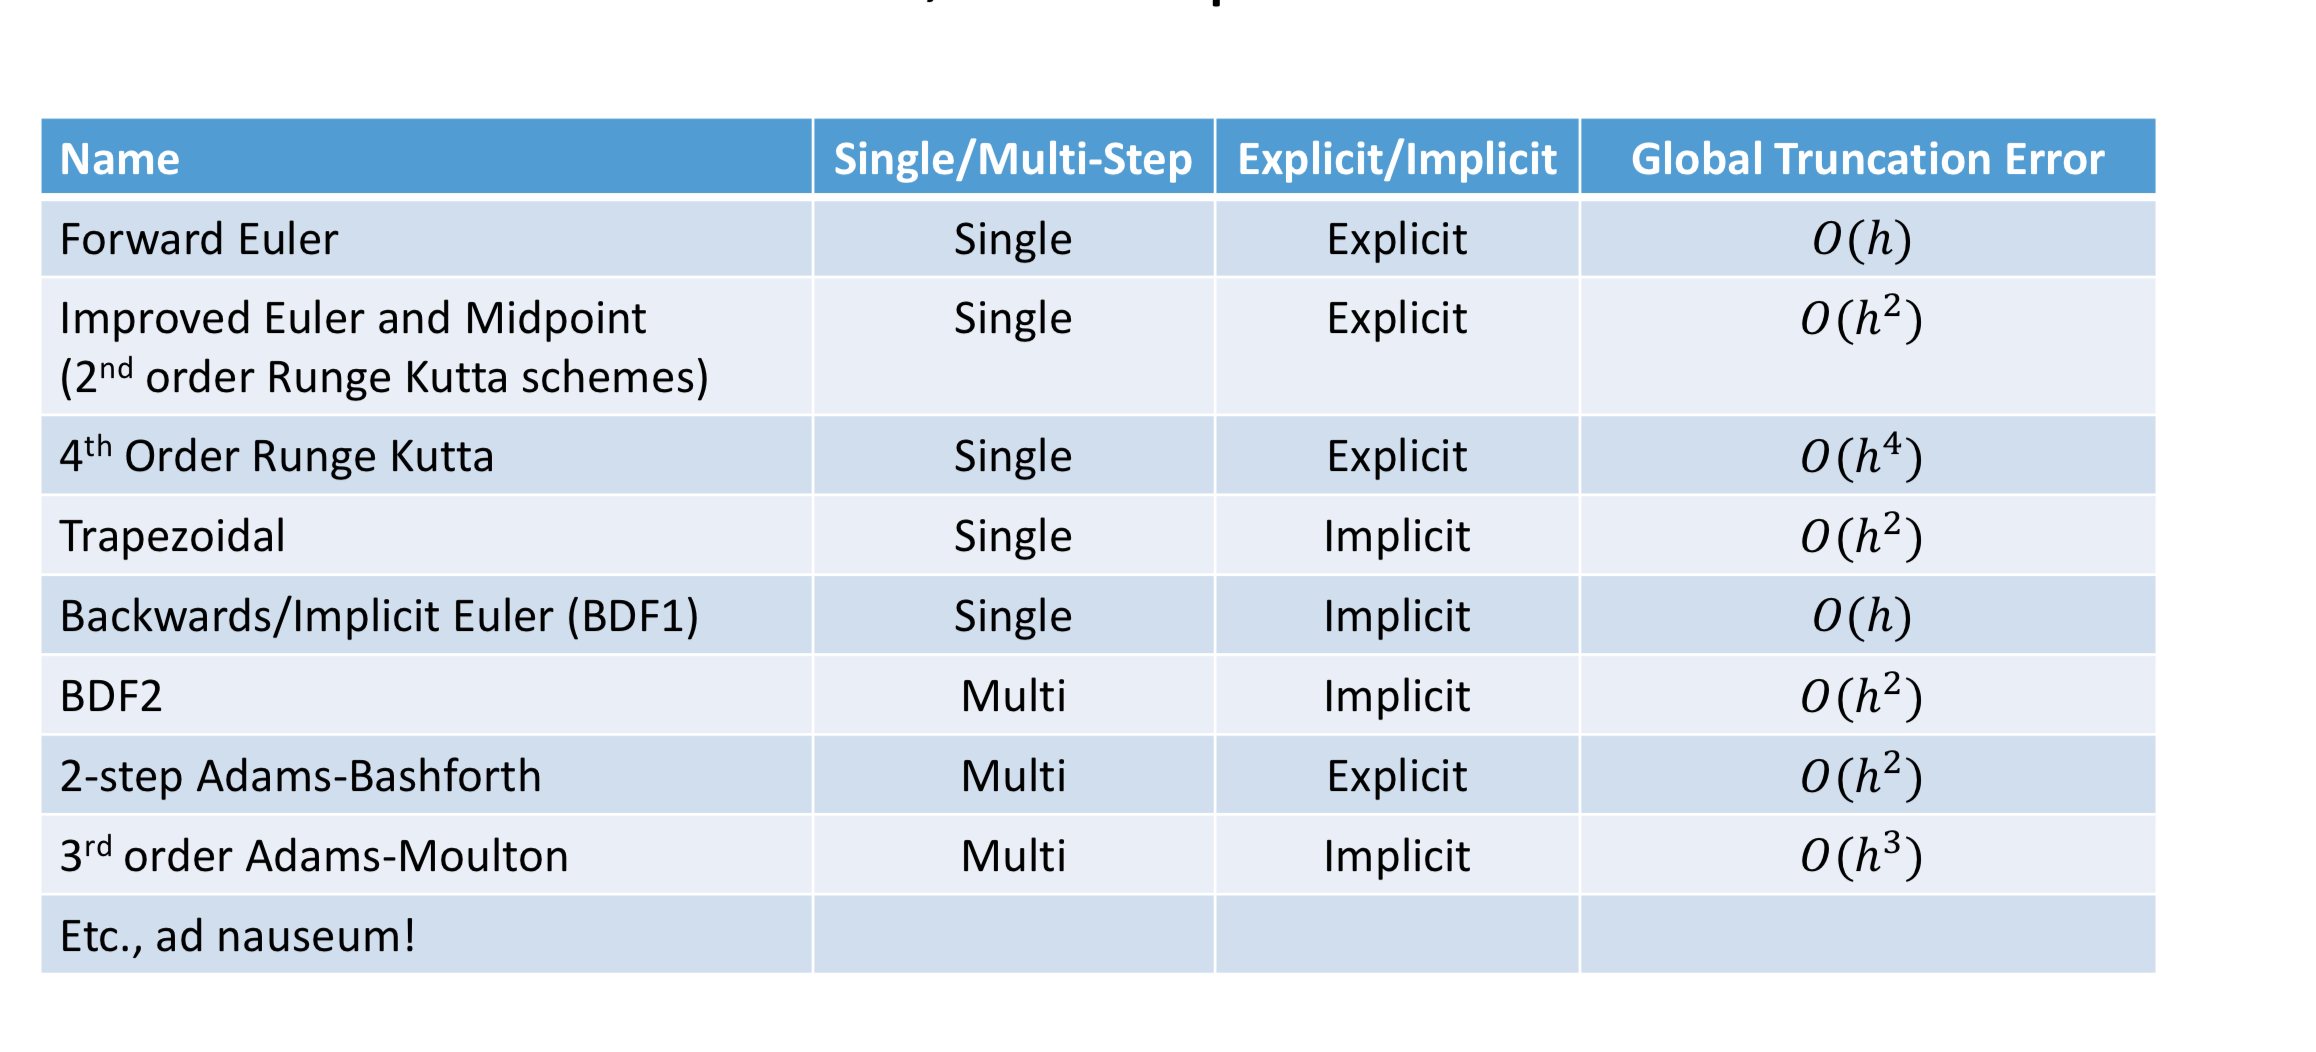
\includegraphics[scale=0.5]{2}
\end{center}

\end{document}




